\steppingstone{Finding Our Way Home}
\label{stone:home}

Until now we have been thinking like builders. A builder reaches a point by adding beams, one at a time, until the construction is complete. The six-beam address remembers that journey.

A surveyor asks a different question.

Where is that point in ordinary three-dimensional space?

The builder and the surveyor are describing the same object. They simply speak different languages.

\section*{From Construction to Position}

Suppose a point has the construction

\[
[a,b,c,d,e,f].
\]

Each number records how many beams were added from one family. The corresponding Cartesian coordinates are obtained by collecting the contributions from the six basis vectors:

\[
\begin{aligned}
x &= \varphi(a+b) + (c-d),\\
y &= (a-b) + \varphi(e+f),\\
z &= \varphi(c+d) + (e-f).
\end{aligned}
\]

Each coordinate is itself an exact PhiBase quantity,

\[
\begin{aligned}
x &= P(c-d,\;a+b),\\
y &= P(a-b,\;e+f),\\
z &= P(e-f,\;c+d).
\end{aligned}
\]

Nothing has been approximated. The six-beam construction and the Cartesian point describe exactly the same place.

\begin{figure}[htbp]
\centering
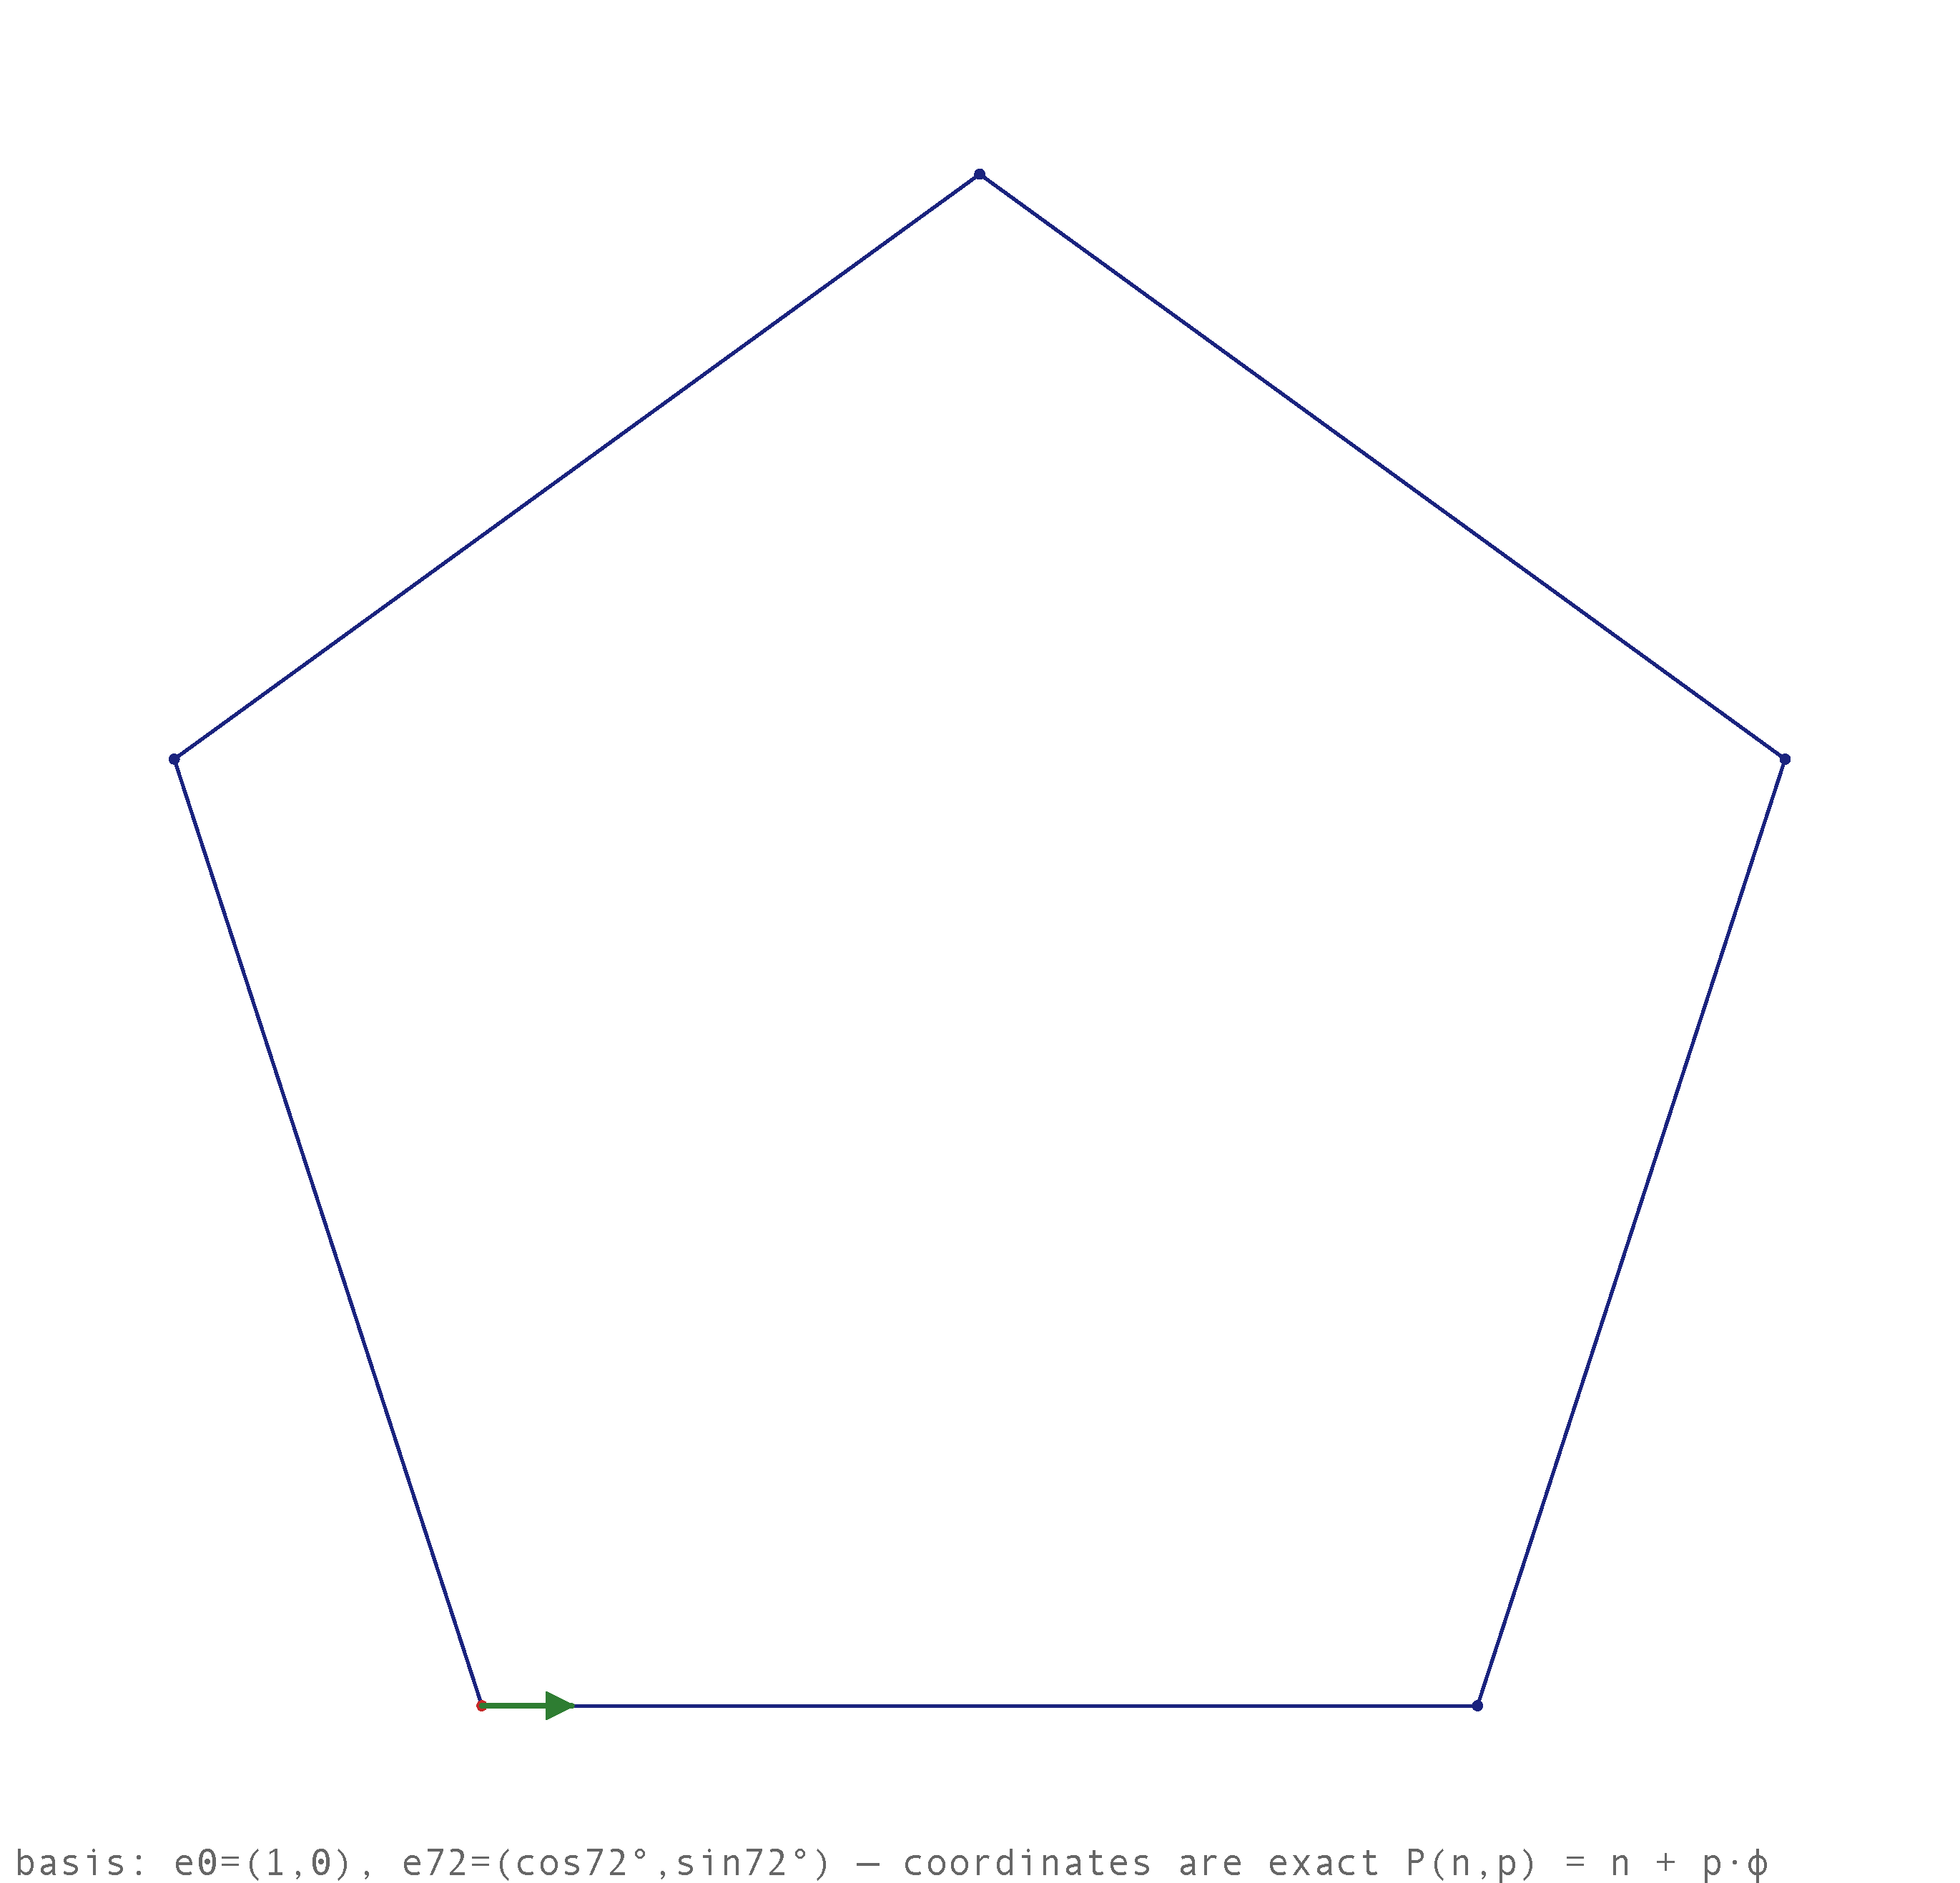
\includegraphics[width=.92\textwidth]{figures/turtle/home.pdf}
\caption{The same point described in two languages. The six-beam address remembers the construction, while the Cartesian coordinates describe its position.}
\label{fig:home}
\end{figure}

\section*{A Small Example}

Begin with the construction

\[
[1,0,0,0,0,0].
\]

Substituting into the three equations gives

\[
(\varphi,\;1,\;0).
\]

One beam has become one point in space.

Now add a second beam from the opposite family:

\[
[1,1,0,0,0,0].
\]

The horizontal contributions reinforce one another while the vertical contributions cancel, giving

\[
(2\varphi,\;0,\;0).
\]

The construction and the coordinates tell the same story from different points of view.

\section*{The Journey Home}

Finding the Cartesian coordinates was never the difficult part.

Can we reverse the process?

Suppose the surveyor hands us

\[
(x,y,z),
\]

where each coordinate has already been written in PhiBase form,

\[
x=P(n_x,p_x),\qquad
y=P(n_y,p_y),\qquad
z=P(n_z,p_z).
\]

Can we recover the six beam counts?

Yes.

Separating the short and long parts of each coordinate gives

\[
\begin{aligned}
a &= \frac{n_y+p_x}{2}, &
b &= \frac{p_x-n_y}{2},\\[1ex]
c &= \frac{n_x+p_z}{2}, &
d &= \frac{p_z-n_x}{2},\\[1ex]
e &= \frac{p_y+n_z}{2}, &
f &= \frac{p_y-n_z}{2}.
\end{aligned}
\]

The original construction quietly returns.

\section*{Nothing Has Been Lost}

Notice what the inverse map uses.

Only addition,

only subtraction,

and division by two.

The journey into Cartesian space looked complicated because six directions became three coordinates. The journey home is simply the process of separating those contributions again.

There is one condition.

Every numerator must be even.

If one numerator is odd, then the point cannot have been assembled from complete beams. The arithmetic tells us immediately whether the construction belongs to the six-beam lattice.

The coordinates remember where the point is.

The beam counts remember how it was built.

Together they describe the same object completely.

\section*{Builder's Notebook}

Translate the constructions

\[
[1,0,0,0,0,0],
\qquad
[1,1,0,0,0,0],
\qquad
[1,0,1,0,1,0]
\]

into Cartesian coordinates.

Then apply the inverse equations and verify that every beam count returns exactly to its original value.

\section*{Looking Ahead}

The journey into space and the journey home are exact inverses of one another. The next question is just as natural.

What happens if the entire construction is reflected in a mirror?
